\begin{frame}
	\frametitle{\tbf{Internships}}

%%%
	\begin{minipage}{0.1\linewidth}
	
	\begin{center} \begin{tabular}{c}
	
\includegraphics[height=1 cm]{logos/logopmc.jpg} \\[2ex]
	%\* \\
	
\includegraphics[width =1.4 cm]{logos/LOMA-CNRS-logo.png} \\[2ex]
	%\* \\
	
\includegraphics[height=1 cm]{logos/Hunan_University_logo.png} \\[2ex]
	%\* \\
	
\includegraphics[height=1 cm]{logos/LCPMR-CNRS-logo.png}
	\end{tabular} \end{center}
	
	\end{minipage}
	%%%
	\begin{minipage}{0.02\linewidth}
	\end{minipage}
	%%%
	\begin{minipage}{0.88\linewidth}
	
	\begin{itemize}
		\setlength{\itemsep}{3pt}

	\item[$\bullet$] \tbf{Probabilistic Approach to Diffusion-mediated Surface Phenomena} \\
	M2S2, Denis Grebenkov \hfill Apr. $\sim$ Jul. 2023 \\
	\small{Laboratoire de Physique de la Matière Condensée, Ecole Polytechnique}

	\normalsize
	\item[$\bullet$] \tbf{Brownian Motion near the Soft Surface} \hfill Feb. $\sim$ Jul. 2022 \\
	M1S2, Thomas Salez, Yacine Amarouchene, David Dean \hfill \textbf{17.40}/20 \\
	\small{Laboratoire Ondes et Matière d’Aquitaine, Université de Bordeaux}
	
	\normalsize
	\item[$\bullet$] \tbf{Study of $\eta^{(\prime)} \to \pi^+ \pi^- \gamma^{(\ast)}$ Decays by Effective Field Theory} \\
	Research Assistant, Lingyun Dai \hfill Mar. $\sim$ Aug. 2021 \\
	\small{School of Physics \& Electronics, Hunan University}
	
	\normalsize
	\item[$\bullet$] \tbf{Simulation of Vibrational ICD on Model Systems with Reduced Dimensions} \hfill Jun. $\sim$ Jul. 2020 \\
	L3S2, Jérémie Caillat \hfill \textbf{15.00}/20 \\
	\small{Laboratoire de Chimie Physique - Matière et Rayonnement, Sorbonne Université}
	
	\end{itemize}


	\end{minipage}
	
	\bigskip
	
	
	%%%
	\begin{minipage}{0.45\linewidth}
	\begin{center}
		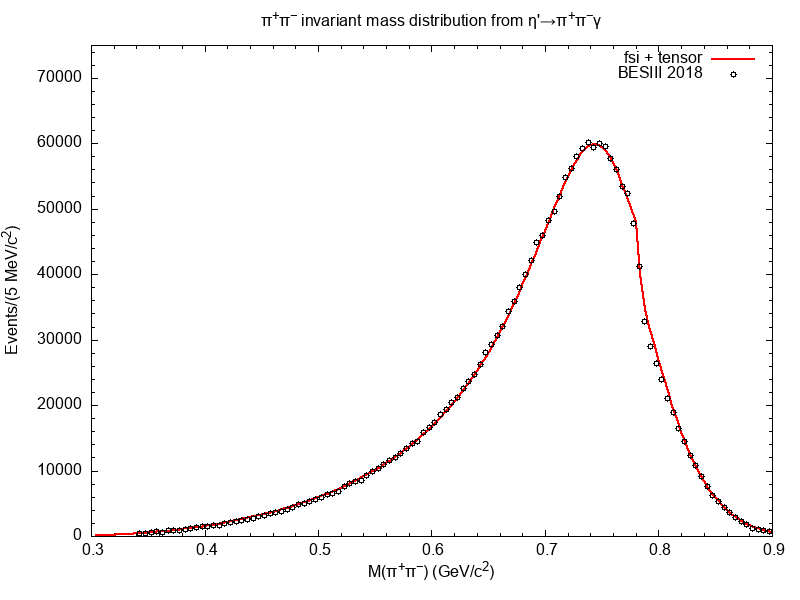
\includegraphics[width = 3.6cm]{figs/spec_pp18_290.png}
	\end{center}
	\end{minipage}
	%%%
	\begin{minipage}{0.1\linewidth}
	\end{minipage}
	%%%
	\begin{minipage}{0.5\linewidth}
	\begin{center}
		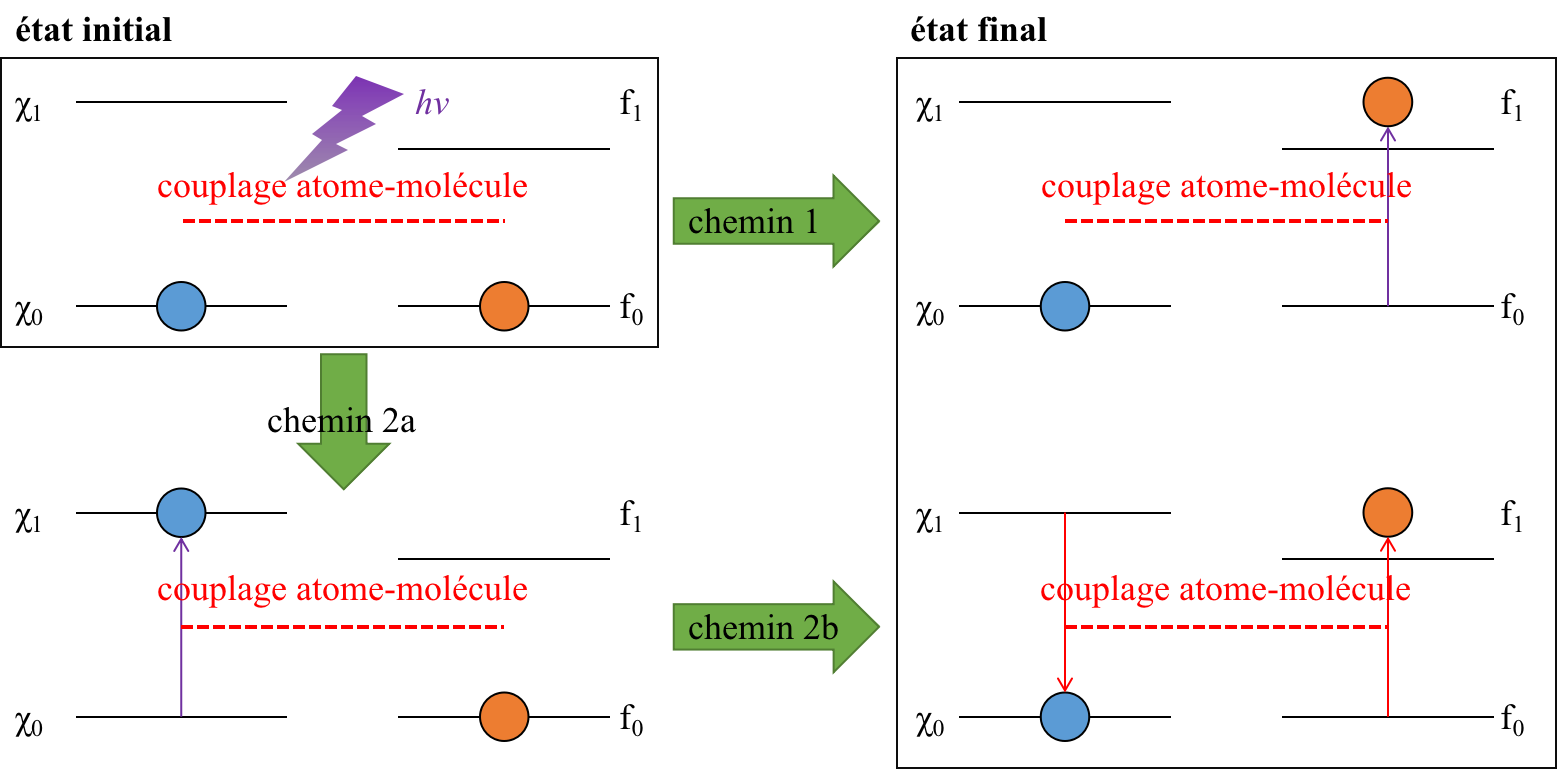
\includegraphics[height = 2.5 cm]{figs/vibicd2.png}
	\end{center}
	\end{minipage}
		
		
	
\end{frame}